\chapter{基本概念}



\section{微分方程及其解的定义}



\begin{exercise}
  验证下列函数是右侧相应微分方程的解或通解:
  \begin{enumerate}[(1)]
  \item $y=C_1\e^{2x}+C_2\e^{-2x}:y''-4y=0$;
  \item $\displaystyle y=\frac{\sin x}{x}:xy'+y=\cos x$;
  \item $y=x\left(\int x^{-1}\e^x\diff x+C\right):xy'-y=x\e^x$;
  \item $y=\begin{cases}-\frac{1}{4}(x-C_1)^2,&-\infty<x<C_1,\\0,&C_1\leq x\leq C_2,\\+\frac{1}{4}(x-C_2)^2,&C_2<x<+\infty,\end{cases}:y'=\sqrt{|y|}$
  \end{enumerate}
\end{exercise}

\begin{proof}
  (1) $y=C_1\e^{2x}+C_2\e^{-2x}\Rightarrow y'=2C_1\e^{2x}-2C_2\e^{-2x}\Rightarrow y''=4C_1\e^{2x}+4C_2\e^{-2x}\Rightarrow y''-4y=0$;

  (2) $y=\frac{\sin x}{x}\Rightarrow y'=\frac{x\cos x-\sin x}{x^2}\Rightarrow xy'+y=\frac{x\cos x-\sin x}{x}+\frac{\sin x}{x}=\cos x$;

  (3) $y=x\left(\int x^{-1}\e^x\diff x+C\right)\Rightarrow y'=\int x^{-1}\e^x\diff x+C+\e^x\Rightarrow xy'-y=x(\int x^{-1}\e^x\diff x+C)+x\e^x-y=x\e^x$;

  (4) 当 $x<C_1$ 时, $y'=-\frac{1}{2}(x-C_1)$,
  而 $\sqrt{|y|}=\sqrt{\frac{1}{4}(x-C_1)^2}=\frac{1}{2}(C_1-x)$,
  故 $y'=\sqrt{|y|}(x<C_1)$, 其他两段同理可以验证.
\end{proof}



\begin{exercise}
  求下列初值问题的解:
  \begin{enumerate}[(1)]
  \item $y'''=x,y(0)=a_0,y'(0)=a_1,y''(0)=a_2;$
  \item $\frac{\diff y}{\diff x}=f(x),y(0)=0$ (这里 $f(x)$ 是一个连续函数);
  \item $\frac{\diff R}{\diff t}=-aR,R(0)=1$ (这里 $a>0$ 是一个常数);
  \item $\frac{\diff y}{\diff x}=1+y^2,y(x_0)=y_0.$
  \end{enumerate}
\end{exercise}

\begin{solve}
  (1) $y(x)=\frac{1}{24}x^4+\frac{a_2}{2}x^2+a_1x+a_0$;

  (2) $y(x)=\int_0^xf(t)\diff t$;

  (3) $R(t)=\e^{-at}$;

  (4) $y(x)=\tan(x+\arctan y_0-x_0)$.
\end{solve}



\begin{exercise}
  求出:
  \begin{enumerate}[(1)]
  \item 曲线族$y=Cx+x^2$所满足的微分方程;
  \item 曲线族$y=C_1\e^x+C_2x\e^x$所满足的微分方程;
  \item 平面上以原点为中心的一切圆所满足的微分方程;
  \item 平面上一切圆所满足的微分方程.
  \end{enumerate}
\end{exercise}

\begin{solve}
  (1) 求导得 $y'=C+2x$, 联立方程消去 $C$ 得 $y+x^2-xy'=0$.

  (2) 求两次导得
  $\begin{cases}y=C_1\e^x+C_2x\e^x\\y'=C_1\e^x+C_2(x+1)\e^x\\y''=C_1\e^x+C_2(x+2)\e^x\end{cases}$, 
  由前两个方程解得 $C_1=\frac{(x+1)y-xy'}{\e^x}$, $C_2=\frac{y'-y}{\e^x}$, 
  代入第三个方程得 $y''-2y'+y=0$.

  (3) 平面上以原点为中心的一切圆的参数方程为 $x^2+y^2=R^2$ ($R$ 为参数), 求导得 $x+yy'=0$.

  (4) 平面上一切圆的参数方程为 $(x-a)^2+(y-b)^2=R^2$ ($a,b,R$ 为参数)
  关于 $x$ 求三次导并消去参数即得 $3y'(y'')^2-\bigl[1+(y')^2\bigr]y'''=0$.
\end{solve}



\begin{exercise}
证明: 设 $y=g(x,C_1,C_2,\cdots,C_n)$ 是一个充分光滑的函数族, 其中 $x$ 是自变量, 
而 $C_1, C_2, \cdots, C_n$ 是 $n$ 个独立的参数(任意常数), 则存在一个形如 (1.1) 的 $n$ 阶微分方程, 
使得它的通解恰好是上述函数族.
\end{exercise}

\begin{proof}
  已知
  \begin{equation}
    \begin{cases}
    y=g(x,C_1,C_2,\cdots,C_n)\\
    y'=g^{(1)}(x,C_1,C_2,\cdots,C_n)\\\cdots\\
    y^{(n-1)}=g^{(n-1)}(x,C_1,C_2,\cdots,C_n)\\
    y^{(n)}=g^{(n)}(x,C_1,C_2,\cdots,C_n)
    \end{cases}\tag{$\star$}
  \end{equation}
  因为 $C_1,C_2,\cdots,C_n$ 独立, 所以 Jacobi 行列式
  \[\frac{D[g,g^{(1)},\cdots,g^{(n-1)}]}{D[C_1,C_2,\cdots,C_n]}=\begin{vmatrix}
  \frac{\partial g}{\partial C_1}&\frac{\partial g}{\partial C_2}&\cdots&\frac{\partial g}{\partial C_n}
  \\
  \frac{\partial g^{(1)}}{\partial C_1}&\frac{\partial g^{(1)}}{\partial C_2}&\cdots&\frac{\partial g^{(1)}}{\partial C_n}\\
  \vdots&\vdots&&\vdots\\
  \frac{\partial g^{(n-1)}}{\partial C_1}&\frac{\partial g^{(n-1)}}{\partial C_2}&\cdots&\frac{\partial g^{(n-1)}}{\partial C_n}\end{vmatrix}\neq 0.\]
  由隐函数存在定理知可由方程组 $(\star)$ 的前 $n$ 个方程解出
  \[C_i=C_i(x,y,\cdots,y^{(n-1)})(i=1,2,\cdots,n).\]
  将之代入方程组 $(\star)$ 最后一个方程中得
  \[y^{(n)}=g^{(n)}(x,C_1(x,y,\cdots,y^{(n-1)}),\cdots,C_n(x,y,\cdots,y^{(n-1)})).\]
  上式即为所求的 $n$ 阶微分方程.
\end{proof}



\section{微分方程及其解的几何解释}



\begin{exercise}
  作出如下微分方程的线素场:
  \begin{enumerate}[(1)]
  \item $\displaystyle y'=\frac{xy}{|xy|}$;
  \item $y'=(y-1)^2$;
  \item $y'=x^2+y^2$.
  \end{enumerate}
\end{exercise}

\begin{solve}
  (1)奇异点集合为 $\{(x,y)\mid x=0\text{\ 或\ }y=0\}$, 线素场如图 (Matlab 制图).
  \begin{figure}[htb]
  \centering
  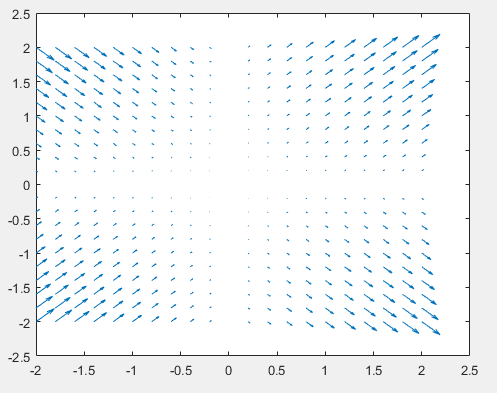
\includegraphics[width=4cm]{figure/ODE1_2_1.png}
  \caption{(1)题图}
  \end{figure}

  (2)等斜线为$(y-1)^2=k\Rightarrow y=1\pm\sqrt{k}$, 线素场如图.
  \begin{figure}[htb]
  \centering
  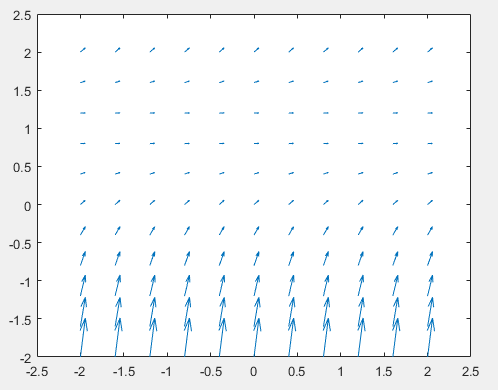
\includegraphics[width=4cm]{figure/ODE1_2_2.png}
  \caption{(2)题图}
  \end{figure}

  (3)等斜线为$x^2+y^2=k$, 线素场如图.
  \begin{figure}[htb]
  \centering
  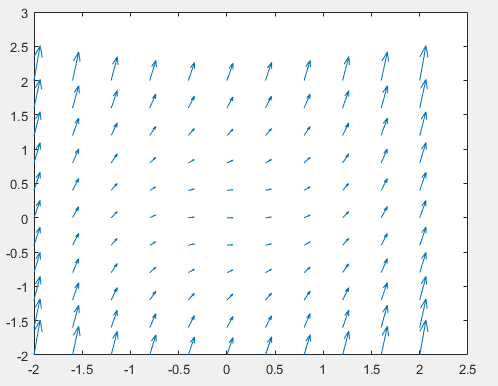
\includegraphics[width=4cm]{figure/ODE1_2_3.png}
  \caption{(3)题图}
  \end{figure}
\end{solve}



\begin{exercise}
  利用线素场研究下列微分方程的积分曲线族:
  \begin{enumerate}[(1)]
    \item $y' = 1+xy$;
    \item $y' = x^2-y^2$.
  \end{enumerate}
\end{exercise}



\begin{exercise}
  根据磁场的物理直观, 试作微分方程 (2.8) 的线素场及其积分曲线族的草图.
\end{exercise}